\chapter{Access Points}

A main component of the project concerns the access points configuration. In
this chapter, their features will be described.

\section{Chained list of the UEs}

The access point will use a chained list in order to save the different
measures retrieved from the UEs' Wi-Fi signals.

With this datastructure the AP is able to manage an infinite number of UEs. For
each of save, it will save its MAC address and its corresponding RSSI value.

It also provides two functions, \emph{build\_element} and \emph{build\_buffer},
that will convert the chained list into JSON data that will be later send to
the Positioning Server.

\section{Passive Sniffer}

Now that the AP has a list, it then needs to fill it with the different values.

In order to find the MAC addresses and the RSSI values of each device, it needs
to sniff the network for any Wi-Fi signals sent by it.

The AP achieve this sniffing by using the \emph{PCAP} library.

It first set up a hook on its interface in order to intercept any Wi-Fi packets
on the network like below.

\begin{figure}[h]
  \centering
  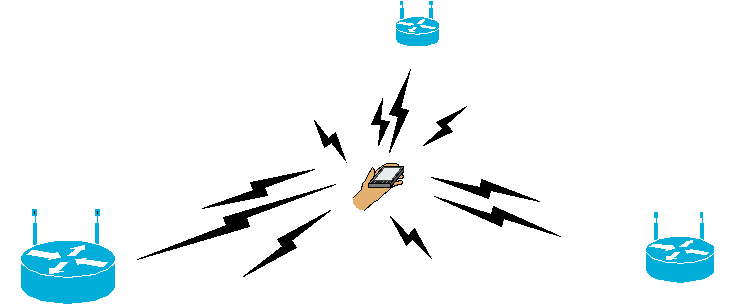
\includegraphics[scale=.5]{./ap/mobile_with_aps.png}
  \caption{Each AP sniffs the Wi-Fi packets of the network}
\end{figure}

Then for each packet, it extracts the MAC address and the RSSI value fields.

\begin{figure}[h]
  \centering
  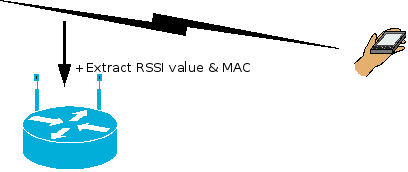
\includegraphics[scale=.7]{./ap/focus_mobile_with_aps.png}
  \caption{For each packet, the AP extracts two fields}
\end{figure}

It sets up a
hook on its interface and extract form the sniffed packets two fields: the MAC
address and the RSSI value.

It then create a new list element with these two values.

\section{HTTP Daemon}

At this point, the AP is able the measure every RSSI values for any devices on
the network. It then has to be able to send them to the Positioning Server when
asked.

Therefore the AP creates a HTTP daemon using the \emph{MicroHTTP} library.

When being fired up, it will initialize that daemon using the
\emph{start\_microhttpd} function. As a callback function, the AP will pass the
\emph{connection\_callback} one that will react to a \emph{?mac=} HTTP request.

It will then uses the list's functions in order to create the JSON response and
sends it to the PS.
